\documentclass{book}

\usepackage{amsmath}
\usepackage{booktabs} % For \toprule, \midrule and \bottomrule.
\usepackage{graphicx}
\usepackage{hyperref} % For hyperlinks.
\usepackage{pgfplots}
\usepackage{pgfplotstable} % Generates table from .csv.
\usepackage{setspace}
\usepackage{siunitx} % Formats the units and values.
\usepackage{subcaption}
\usepackage{tikz} % To generate the plot from csv.
\usepackage{titlepic}

\pgfplotsset{compat=newest} % Allows to place the legend below plot.
\usepgfplotslibrary{units} % Allows to enter the units nicely.

% Round numbers to 2 places.
\sisetup{
  round-mode = places,
  round-precision = 2,
}

%\setcounter{tocdepth}{1} % Show sections.
%\setcounter{tocdepth}{2} % + subsections.
\setcounter{tocdepth}{3} % + subsubsections.
%\setcounter{tocdepth}{4} % + paragraphs.
%\setcounter{tocdepth}{5} % + subparagraphs.

\graphicspath{ {images/} }

\title{This is a title}
\author{This is an author}
\titlepic{
\includegraphics[width=5cm]{polimi}}
\date{\vspace{-5ex}}

\begin{document}

\pagenumbering{gobble}

\maketitle

\pagenumbering{roman}

\cleardoublepage
\newpage

\doublespacing % Double the spacing for the ToC.
\tableofcontents
\singlespacing % Reset the spacing.

\cleardoublepage
\newpage

\listoffigures

\cleardoublepage
\newpage

\listoftables

\cleardoublepage
\newpage

\pagenumbering{arabic}

\section{Introduction}

This is a section.

\subsection{Subsection}

This is a subsection.

\paragraph{Paragraph} 

This is a paragraph in a subsection.

\subparagraph{Subparagraph} 
 
This is a subparagraph in a subsection.

\section{Math}

This section contains an equation:

\begin{equation}
f(x) = x^2 + 2
\end{equation}

If you don't want your equation to be numbered, use *:

\begin{equation*}
f(x) = x^2 + 2
\end{equation*}

Moreover, equations can be aligned:

\begin{align*}
f(x) &= x^2\\
g(x) &= \frac{1}{x}\\
g(x) &= \frac{1}{\sqrt{x}} \\
F(x) &= \int^a_b \frac{1}{3}x^3
\end{align*}

I can also have math embedded in a text delimited by the \$ sign, like this: $f(x) = x^2 + 2$ .

\paragraph{} 

Finally, we have a matrix:

\begin{equation*}
\left[
\begin{matrix}
1 & 0\\
0 & 1
\end{matrix}
\right]
\end{equation*}

The left and right notation is used to scale the brackets, but can also be used with other elements. 

\section{Figures}

\begin{figure}
  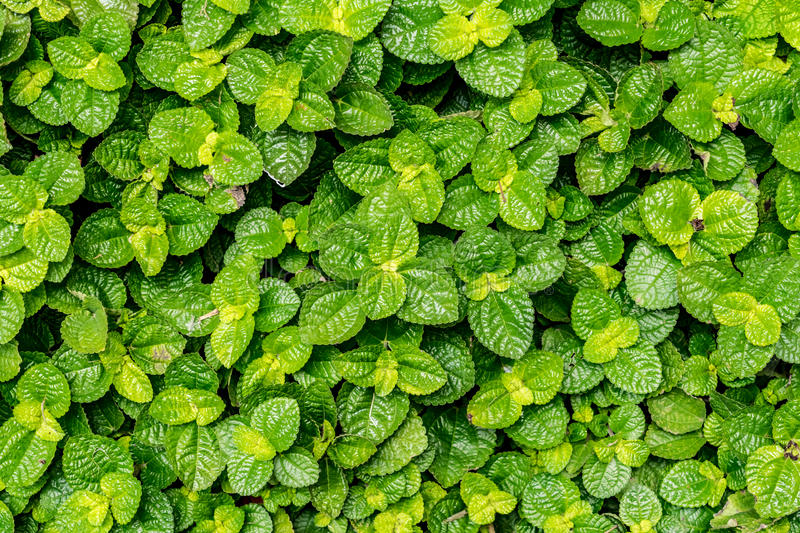
\includegraphics[width=\linewidth]{mint.jpg}
  \caption{Some mint.}
  \label{fig:mint1}
\end{figure}

Figure \ref{fig:mint1} shows some mint.

\begin{figure}[ht!]
  \centering
  \begin{subfigure}[b]{0.4\linewidth}
    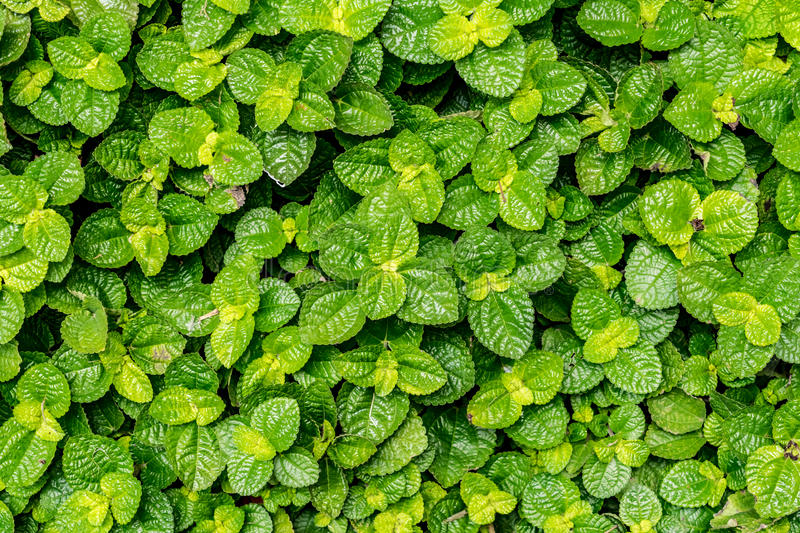
\includegraphics[width=\linewidth]{mint.jpg}
    \caption{Mint.}
  \end{subfigure}
  \begin{subfigure}[b]{0.4\linewidth}
    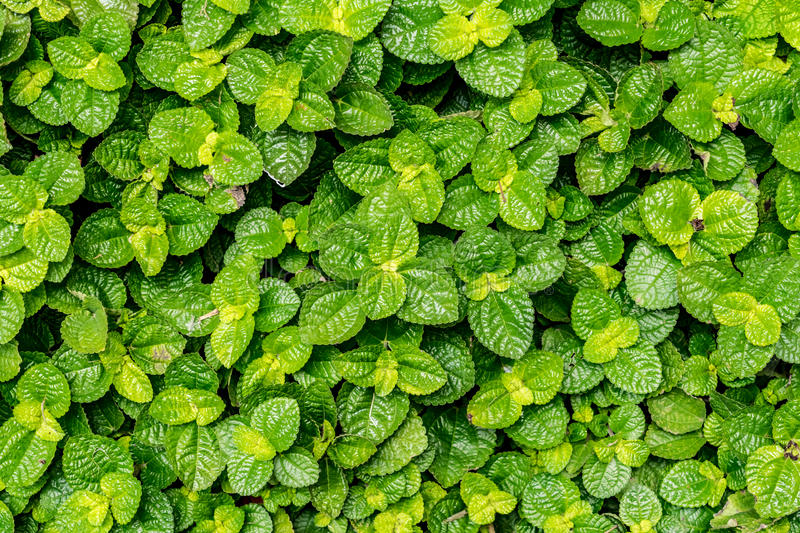
\includegraphics[width=\linewidth]{mint.jpg}
    \caption{More mint.}
  \end{subfigure}
  \caption{The same mint. Twice.}
  \label{fig:mints1}
\end{figure}

\paragraph{} 

Figure \ref{fig:mints1} shows even more mint. Here I have set linewidth to .4 instead of 0.5 ($0.5 * 2 = 1$), since you always have to set it .1 less than you expect.

\begin{figure}[ht!]
  \centering
  \begin{subfigure}[b]{0.2\linewidth}
    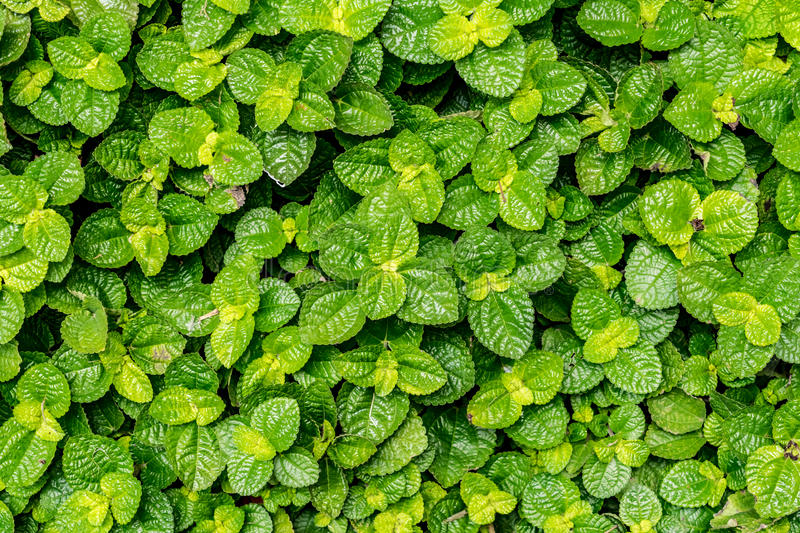
\includegraphics[width=\linewidth]{mint.jpg}
     \caption{Mint.}
  \end{subfigure}
  \begin{subfigure}[b]{0.2\linewidth}
    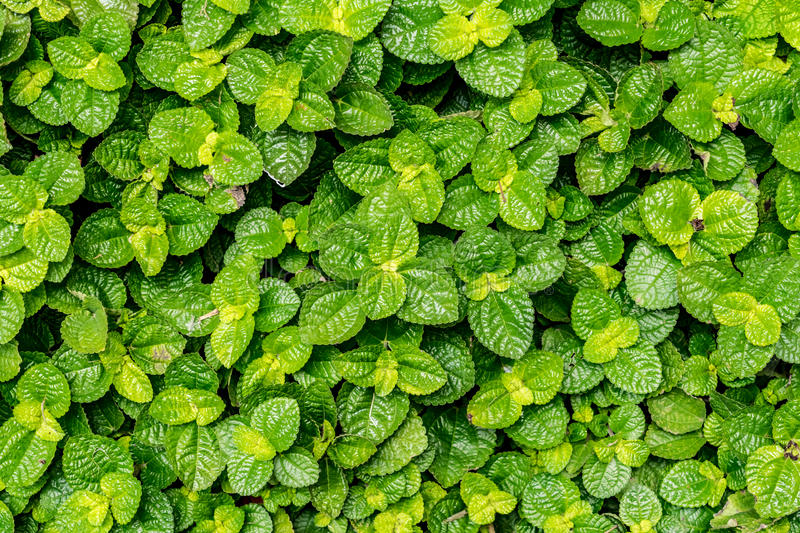
\includegraphics[width=\linewidth]{mint.jpg}
    \caption{More mint.}
  \end{subfigure}
  \begin{subfigure}[b]{0.2\linewidth}
    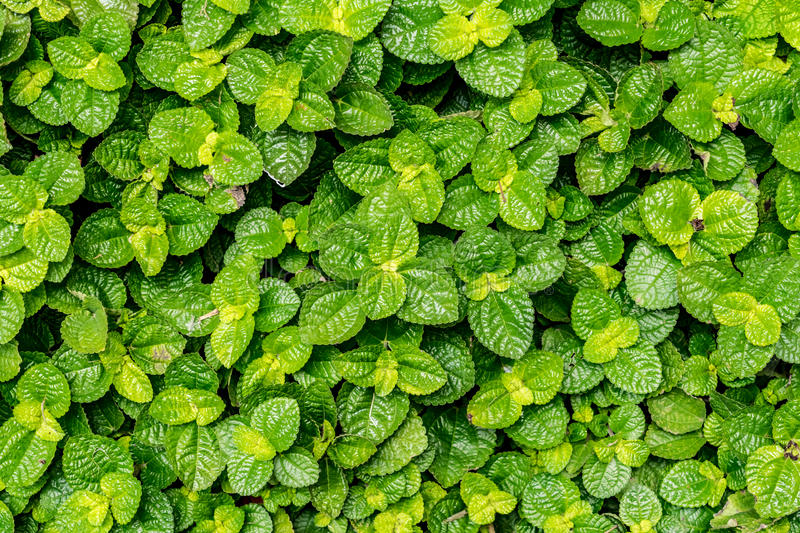
\includegraphics[width=\linewidth]{mint.jpg}
    \caption{Fresh mint.}
  \end{subfigure}
  \begin{subfigure}[b]{0.5\linewidth}
    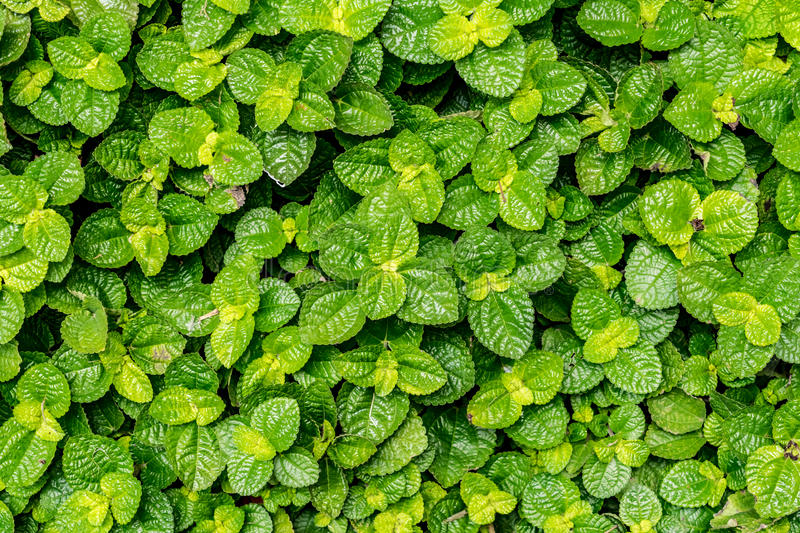
\includegraphics[width=\linewidth]{mint.jpg}
    \caption{Too much mint.}
  \end{subfigure}
  \caption{The same mint. Multiple times. Fresh as ever.}
  \label{fig:mints2}
\end{figure}

\paragraph{} 

Figure \ref{fig:mints1} shows a lot of mint on multiple rows.

\addtocontents{toc}{\setcounter{tocdepth}{1}} % Set depth to 1.
\section{Section which subsections and subsubsections I want to hide in the ToC}

This is a section.

\subsection{Hidden subsection in the ToC}

This is a subsection.

\subsubsection{Hidden subsubsection in the ToC}

This is a subsubsection.

\addtocontents{toc}{\setcounter{tocdepth}{3}} % Reset the depth to default.
\section{Section which subsections and subsubsections I want to show in the ToC}

This is a section.

\subsection{Visible subsection in the ToC}

This is a subsection.

\subsubsection{Visible subsubsection in the ToC}

This is a subsubsection.

\section{Citations and footnotes}

This is a random citation \cite{DUMMY:1} embeddeed in text.

\paragraph{}

This is some example text\footnote{\label{myfootnote}Hello footnote}.

\paragraph{}

I'm referring to footnote \ref{myfootnote}.

\section{Tables}

\begin{table}[ht!]
  \begin{center}
    \caption{A table.}
    \label{tab:table1}
    \begin{tabular}{l|S|r} % Left, centered with aligned decimal points and rigth.
	\toprule
      \textbf{Value 1} & \textbf{Value 2} & \textbf{Value 3}\\
      $\alpha$ & $\beta$ & $\gamma$ \\
      \hline
      1 & 1110.1 & a\\
      2 & 10.1 & b\\
      3 & 23.113231 & c\\
       \bottomrule
    \end{tabular}
  \end{center}
\end{table}

\begin{table}[ht!]
  \begin{center}
    \caption{An autogenerated .csv table.}
    \label{table2}
    \pgfplotstabletypeset[
      multicolumn names, % Allows to have multicolumn names.
      col sep=comma, % The seperator in our .csv file.
      display columns/0/.style={
		column name=$Value 1$, % Name of first column.
		column type={S},string type},  % Use siunitx for formatting.
      display columns/1/.style={
		column name=$Value 2$,
		column type={S},string type},
      every head row/.style={
		before row={\toprule}, % Have a rule at top.
		after row={
			\si{\ampere} & \si{\volt}\\ % The units seperated by &.
			\midrule} % Rule under units.
			},
		every last row/.style={after row=\bottomrule}, % Rule at bottom.
    ]{CSVs/table.csv} % Filename/path to file.
  \end{center}
\end{table}

\section{Plots}

\begin{figure}[ht!]
  \begin{center}
    \begin{tikzpicture}
      \begin{axis}[
          width=\linewidth, % Scale the plot to \linewidth
          grid=major, % Display a grid
          grid style={dashed,gray!30}, % Set the style
          xlabel=X Axis $U$, % Set the labels
          ylabel=Y Axis $I$,
          x unit=\si{\volt}, % Set the respective units
          y unit=\si{\ampere},
          legend style={at={(0.5,-0.2)},anchor=north}, % Put the legend below the plot
          x tick label style={rotate=90,anchor=east} % Display labels sideways
        ]
        \addplot 
        % add a plot from table; you select the columns by using the actual name in
        % the .csv file (on top)
        table[x=column 1,y=column 2,col sep=comma] {CSVs/table.csv}; 
        \legend{Plot}
      \end{axis}
    \end{tikzpicture}
    \caption{My first autogenerated plot.}
  \end{center}
\end{figure}

\section{Hyperlinks}

This is my link: \href{http://www.latex-tutorial.com}{LaTeX-Tutorial}.

\paragraph{}

You can also link to bare URLs without an additional description: \url{http://www.latex-tutorial.com}.

\paragraph{}

My email address is: \href{mailto:claudio.vellage@latex-tutorial.com}{claudio.vellage@latex-tutorial.com}

\section{Lists}

Unordered list:
\begin{itemize}
	\item One
	\item Two
	\item Three
\end{itemize}

\paragraph{}

Ordered list:
\begin{enumerate}
	\item One
	\item Two
	\item Three
\end{enumerate}

\paragraph{}

Nested lists:

\begin{enumerate}
        \item One
    \begin{enumerate}
        \item Two
        \item Three
        \item Four
    \end{enumerate} 
        \item Five
        \item Six
\end{enumerate}

\paragraph{}

Customized list:

\begin{itemize}\item[--] Dash
    \item[-] Dash
    \item[*] Asterisk
\end{itemize}

\newpage
\cleardoublepage

\bibliography{bibliography/bibliography} 
\bibliographystyle{ieeetr}

\end{document}